\documentclass[a4paper]{article}
\usepackage[left=0.5in,top=0.5in,right=0.5in,bottom=0.5in]{geometry} % Document margins

\usepackage{listings}
\usepackage{mathtools}
\usepackage{amsmath,amsfonts,amssymb}
\usepackage{dirtree}
\usepackage{multicol}
\usepackage{tikz}
\usepackage{tcolorbox}
\usepackage{tkz-graph}
\tcbuselibrary{breakable}

\usetikzlibrary{arrows}
\title{SOFTENG 250 Summary Notes (LN 1-10)}
\author{Edward Zhang}
\date{\today}

\lstset{
	basicstyle=\footnotesize\fontfamily{lmss}\selectfont,
	backgroundcolor=\color{black!5},
	escapeinside=||,
	frame = single,
	framexleftmargin=5pt,
	framexrightmargin=5pt,
	keywordstyle=\color{red},
	keywordstyle={[2]\color{blue}},
	keywords={,x, b, c, i, c2, q, r, v, s},
	keywords={[2],if, while, else, set, endif, endwhile, return, for, foreach}
}

\newenvironment{algorithm}[3]{ % name, problem, lecture notes
	\vspace{0.5em}
	\noindent{\Large\bf #1 }{\Large- #2} \hfill {\Large\bf LN#3}
	  \begin{list}{$\bullet$}{\leftmargin=1em}
	}{
	\end{list}
	\vspace{0.5em}
}


\begin{document}
\maketitle
\begin{algorithm}{Gale-Shapely Algorithm}{Stable Matching Problem}{1}
	\item Using the company - applicants matching example, the company ranks all applicants in order of preference and the applicants do the same for companies.
	\item Initially all companies and applicants are free.
	\begin{lstlisting}
while there is a free company (c)
	set x to be c's highest ranked applicant to whom c hasn't made an offer yet
	if x is free then (c, x) becomes a job pair
	else this means x is already in an job pair with c2
		if x prefers c2 to c then c remains free
		else x prefers c to c2 then (c, x) becomes a job pair and c2 becomes free
	endif
endwhile
return the |set| of pairs we generated
	\end{lstlisting}
	\item Due to the dynamically changing size of eg. free companies, a (doubly) linked list is appropriate.
	\item Running time is linear to the size of the input (where the size of the input is number of companies $\times$ number of applicants).
\end{algorithm}
\begin{algorithm}{MergeSort}{Array Sorting}{2}
	\item The Merge algorithm combines two sorted lists in one pass. It keeps a pointer on each list and appends the smaller of the two onto the output list, then advances that pointer.
	\item MergeSort recursively splits the input array in half until size $\leq1$ then recursively combines them using Merge, runs in $O(n\log(n))$ time.
\end{algorithm}
\begin{algorithm}{FindMin}{Finds minimum value of array}{2}
	\item Trivial. Makes one pass through the array while storing the current minimum. Runs in linear time.
\end{algorithm}
\begin{algorithm}{Closest Pair (Brute Force)}{Finds the two closest points in space}{2}
	\item Loop through all points. For each point, loop through all points except itself and compute the distance between them. If this is lower than the currently stored minimum distance, store these points as the new closest pair.
	\item Runs in $O(n^2)$ time, as there is a nested forloop, each of size $n$.
\end{algorithm}
\begin{algorithm}{Disjoint Subset}{Given a set of subsets, Find two subsets with 0 overlap}{2}
	\item Loop through all subsets. For each subset, loop through all other subsets. For each point in the first subset, check if it belongs in the second subset. If no points belong in the second subset then output these two subsets as disjoint.
	\item If each set has a max size of $n$, the inner loop makes $n$ iterations. The loop for the second subsets loops $n$ times. The loop for the outer subsets loops $n$ times too. Hence $O(n^3)$.
\end{algorithm}
\begin{algorithm}{Euclidean Algorithm}{Find Greatest Common Denominator}{2}
	\item First we divide the larger number by the smaller one and find the remainder. Then we divide the smaller number by the remainder then the old remainder by the new remainder until the remainder = 0.
	\item Let b be the larger of the two numbers, and c the smaller one.
	\begin{lstlisting}
while remainder > 0
	find r = x%c (remainder/mod)
	set x = c and c = r
endwhile
return c
	\end{lstlisting}
\end{algorithm}
\begin{tcolorbox}
	\section*{Efficiency and Running Time\hfill{LN3}}
	\begin{quote}
		\centering
		{\Large``An algorithm is efficient if its running time\\ is bounded by a polynomial.''}
	\end{quote}
$O(a)$ represents a asymptotic upper bound, whereas $\Omega(b)$ represents a asymptotic lower bound. $\Theta(c)$ represents a asymptotically tight bound. This is true if $a = b = c$.\\\newline
Log functions are growing functions with a \emph{very slow growth rate}. This function grows much slower than any polynomial. We can see the slow growth rate if we calculate the rise/run. $\frac{\log_b(n)}{n}$ as n approaches infinity is zero, hence the steepness approaches zero. For running time analysis, the base of the log is not considered.\\\newline
Polynomial bounds are of the form $a_0 + a_1n + a_2n^2 + ... + a_nn^k$. The tight bound for this is $\Theta (n^k)$.  Running times can also be bounded by functions like $n^x$ where $x>0$ is \emph{not necessarily a integer}. For instance, you can have an algorithm with a running time bounded by $n^{0.001}$ or $n^{0.57}$. Note that logarithms like $n\log(n)$ are still polynomial since they're upper bounded by $O(n^2)$. Further examples of polynomial bounds (from the test) include;
	\begin{multicols}{2}
		\begin{itemize}
			\item $O(n)$, since this is essentially $O(n^1)$
			\item $O(\sqrt{n^3})$, as this is $O(n^\frac{3}{2})$
			\item $\Theta(n^2\times\log^3(n))$, as $n^2$ is the dominant value
			\item $O(n^4 + n^3.5 + \log^2(n))$, still bound by $n^4$
			\item $O(1)$, basically $O(n^0)$
		\end{itemize}
	% TODO: Add negating examples
	\end{multicols}
An exponential function is in the form of $r^n$, where $r > 1$. Just as log functions are upper bounded by polynomials, polynomials are upper bounded by exponentials: $n^x = O(r^n)$. However unlike Logarithmic functions, we cannot ignore the size of $r$.\\\newline
Some algorithms run in sub-linear time. How can the running time be smaller than the time required to read the input of size $n$? Sub-linear time algorithms \emph{do not read the entire input}. A good example is Binary Search, below.
\end{tcolorbox}
\vspace{1em}
\begin{algorithm}{Binary Search}{Find if $x$ is in a sorted array}{3}
	\item Brute force completes this in linear time. However Binary Search is faster, given a sorted array.
	\item Find the mid point. If it's x, we're done. Otherwise, compare the midpoint to x to determine whether x is in the upper half or lower half of the array. This halves the search space. We now find the mid point again etc. etc. until x is found or if we run out of entries to check.
	\item At each step, the search space is halved. Therefore after $k$ steps the search space is $0.5^kn$. Therefore, the number of times we halve the segments is $\leq\log(n)$, thus the running time is $O(\log(n))$, which is sublinear time.
\end{algorithm}
\begin{tcolorbox}[breakable]
	\section*{Graph Definitions\hfill{LN4}}
	\begin{itemize}
		\item \emph{Undirected Graphs} are also just simply known as \emph{graphs}. They are the most basic type of graphs and consist of points \emph{(vertices)} and lines \emph{(edges)}. Edges that connect a vertex to itself are disallowed. Multiple edges between any two vertices are also disallowed.
		\item \emph{Vertices} are points on the graph to which edges connect. The set of vertices of a graph are written like $V = \{0, 1, 2, 3, ..., 9\}$
		\item \emph{Edges} are the lines that connect multiple vertices. For example a series of edges between vertices 0 and 1, 0 and 3 and 2 and 3 can be written as $E = \{\{0,1\}\{0,3\}\{2,3\}\}$
		\item \emph{Degrees} are the number of edges connected to a vertex; so a vertex with 4 edges connect to it would have a degree of 4.
		\item \emph{Digraphs (Directed Graphs)} still consists of points \& edges, however the edges have specific directions (ie. they're arrows). For example a series of edges from vertices 0 to 1, 0 to 3 and 2 to 3 can be written as $E = \{(0,1)(0,3)(2,3)\}$
		\item \emph{Complete} graphs are graphs where every vertex is directly connected to every other vertex.
		\item \emph{A path} is a sequence of vertices such that $\{v_0, v_1\}, \{v_1, v_2\}, \{v_{n-1}, v_n\}$ etc., thus forming a \emph{path} from $0$ to $n$. $n$ is regarded as the length of this path. Paths are reversible (ie. starting at $n$ and ending at $0$) (except for in digraphs).
		\item \emph{Connectivity}: Vertices $u$ and $v$ are connected if there is a path from $u$ to $v$. Note every vertex is connected to itself. A \emph{component} of vertex $v$ is the collection of all vertices that are connected to $v$. A entire graph $G$ is connected if all pairs of $u$ and $v$ are connected.
		\item \emph{Strong Connectivity}: Where vertex $u$ has a path to $v$ and $v$ also has a path back to $u$. Only relevant for digraphs.
		\item \emph{Cycles} are paths where no vertices are repeated except the start and finish being the same vertex.
		\item \emph{Trees} are graphs that are connected and contain no cycles. We call vertices in a tree nodes.
		\item Rooting a tree is when we select a vertex in a tree and ``pull it up'' and let the rest of the vertices ``dangle down''. This vertex is the root of the tree and we move down from the root to the leaves. The parent of a node $v$ is $u$ where we encounter $u$ first then $v$ on it's path from $r$.
	\end{itemize}
\end{tcolorbox}
\begin{tcolorbox}[breakable]
	\section*{Graph Arrangements\hfill{LN4}}
	Note that these examples are directed, however undirected versions exist too.
	\begin{multicols}{2}
		\subsubsection*{Cycles}
		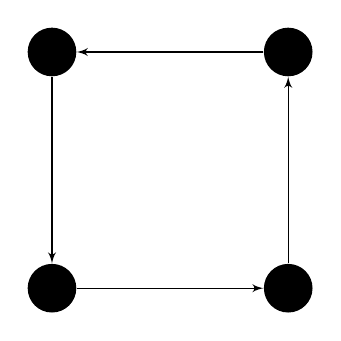
\begin{tikzpicture}
		[scale=1,auto=center,every node/.style={circle,fill=black},edge/.style={->,> = latex'}]
		\node (n4) at (1,1)  {4};
		\node (n3) at (1,4)  {3};
		\node (n1) at (4,1) {1};
		\node (n2) at (4,4)  {2};
		
		\foreach \from/\to in {n1/n2,n2/n3,n3/n4,n4/n1}
		\draw[edge] (\from) -- (\to);
		\end{tikzpicture}\\
		A cycle of length $n$ has $n$ vertices and $n$ edges, arranged as $(0,1) (1,2), (2,3), ..., (n-1, 0)$.
		\columnbreak
		\subsubsection*{Wheels}
		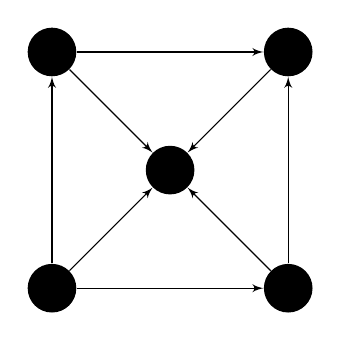
\begin{tikzpicture}
		[scale=1,auto=center,every node/.style={circle,fill=black},edge/.style={->,> = latex'}]
		\node (n5) at (2.5,2.5) {5};
		\node (n4) at (1,1)  {4};
		\node (n3) at (1,4)  {3};
		\node (n1) at (4,1) {1};
		\node (n2) at (4,4)  {2};
		
		\foreach \from/\to in {n1/n2,n3/n2,n4/n3,n4/n1,n1/n5,n2/n5,n3/n5,n4/n5}
		\draw[edge] (\from) -- (\to);
		\end{tikzpicture}\\
		A wheel of size $n$ (where $n > 2$) has $n$ vertices and $2n$ edges, arranged as $(1,2), (2,3), ..., (n-1, 1)$ and $(1,0), (2,0), (n,0)$ (0 is in the center)
	\end{multicols}
	\begin{multicols}{2}
		\subsubsection*{Grids}
		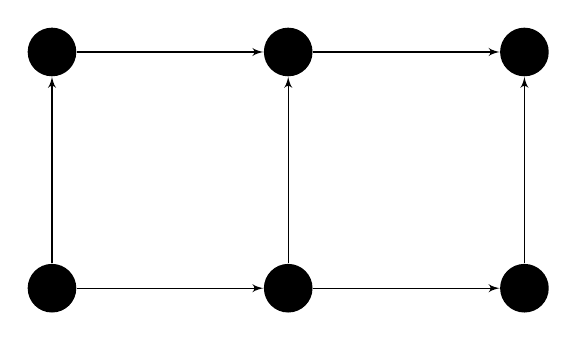
\begin{tikzpicture}
		[scale=1,auto=center,every node/.style={circle,fill=black},edge/.style={->,> = latex'}]
		\node (n4) at (1,1)  {4};
		\node (n3) at (1,4)  {3};
		\node (n1) at (4,1) {1};
		\node (n2) at (4,4)  {2};
		\node (n5) at (7,1) {5};
		\node (n6) at (7,4) {6};
		
		\foreach \from/\to in {n1/n2,n3/n2,n4/n3,n4/n1,n1/n5,n2/n6,n5/n6}
		\draw[edge] (\from) -- (\to);
		\end{tikzpicture}
		\columnbreak
		\subsubsection*{Cubes}
		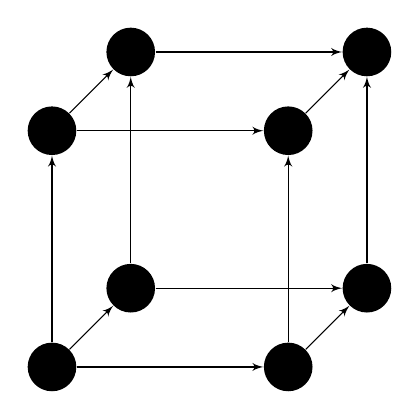
\begin{tikzpicture}
		[scale=1,auto=center,every node/.style={circle,fill=black},edge/.style={->,> = latex'}]
		\node (n8) at (2,2)  {8};
		\node (n7) at (2,5)  {7};
		\node (n5) at (5,2) {5};
		\node (n6) at (5,5)  {6};
		\node (n4) at (1,1)  {4};
		\node (n3) at (1,4)  {3};
		\node (n1) at (4,1) {1};
		\node (n2) at (4,4)  {2};
		
		\foreach \from/\to in {n1/n2,n3/n2,n4/n3,n4/n1,n5/n6,n7/n6,n8/n7,n8/n5,n4/n8,n3/n7,n2/n6,n1/n5}
		\draw[edge] (\from) -- (\to);
		\end{tikzpicture}
	\end{multicols}
\end{tcolorbox}
\vspace{1em}
\begin{algorithm}{BFS algorithm}{Construct the component of $s$}{5}
	\item We start at $s$ and we define $L_0$ (Layer 0) as just ${s}$. We then proceed to store all vertices adjacent to members of $L_0$ (ie. vertices adjacent to $s$) into $L_1$. Then we store all vertices adjacent to all members of $L_1$ into $L_2$ and so on and so forth.
	\item We can implement BFS using the Queue data structure (FIFO). We pop the oldest vertex from the queue and find all of it's adjacent vertices. We then put these vertices into the back of the queue. We will need a separate array to store vertices that we've already explored to avoid duplicates.
	\item Generates a BFS-Tree, runs in $O(n + m)$ time, where $n$ is the number of vertices and $m$ is the number of edges.
\end{algorithm}
\begin{algorithm}{DFS algorithm}{Construct the component of $s$}{5}
	\item We start at $s$ and we ``walk'' along the edges until we reach a dead end. From there we backtrack until we find a vertex that has unexplored edges and we then ``walk'' along those edges, and son on and so forth.
	\item We can implement BFS using the Stack data structure (LIFO). We pop a vertex from the Stack and replace it with all of it's adjacent vertices. Now we pop one of these vertices and put all of it's adjacent vertices etc. We will need a separate array to store vertices that we've already explored to avoid duleplicates.
	\item Generates a DFS-Tree, also runs in $O(n + m)$ time.
\end{algorithm}
\begin{algorithm}{Strong Connectivity}{Check if digraph $G$ is strongly connected}{6}
	\item Run BFS on $G$, then reverse all vertices in $G$ and construct BFS again. If both BFS outcomes are identical, then $G$ is strongly connected.
\end{algorithm}
\begin{tcolorbox}
	\section*{DAGs and Topological Order\hfill{LN6}}
Consider a set of tasks that represent the set of courses needed to complete a SE degree with dependency relations between these tasks (ie. We must complete course $a$ before doing $b$): This can be represented by a directed acyclic graph (or DAG). There have a different structure from acyclic undirected graphs (which are just trees). A topological order would represent an order the courses can be completed in without creating any conflicts (ie. once we get to course $c$ in the order all of it's prerequisites have already been completed earlier on in the order).\\\newline
In-degrees and out-degrees are like degrees for undirected graphs except in-degrees represent edges going into a vertex and out-degrees represent edges coming out of a vertex.
\end{tcolorbox}
\vspace{1em}
\begin{algorithm}{Topological Order}{Finds the topological order of a DAG $G$}{6}
	\item By definition a DAG must have at least one vertex with an in-degree of zero (otherwise there will be a cycle)
	\item While $G$ is not empty, find a vertex with an in-degree of zero and append it to the output, then delete this vertex from $G$. Now find the next vertex with an in-degree of zero etc.
	\item Using a basic implementation, running time is $n^2$ as it takes $n$ time to \emph{find} and delete a vertex from the graph and the while loop makes $n$ iterations.
	\item However, if when a vertex $v$ is removed we decrease the in-degree of those it is adjacent to while simultaneously checking to see of the in-degree of these have decreased to 0, we can achieve a better running time since we don't have to check $n$ every iteration, instead just every outbound edge of $v$. This means that each edge is only checked once, and thus the running time is $O(n + m)$ with the implementation.
\end{algorithm}
\begin{tcolorbox}[breakable]
	\section*{Greedy Algorithms \& Scheduling Problems\hfill{LN7}}
	Greedy Algorithms build the solution step by step and are defined as;
		\begin{quote}
		\centering
		{\Large``An algorithm that makes the locally optimal choice at each stage\\in order to find the global optimum''}
	\end{quote}
	We define requests in a scheduling problem in the following form;
	\begin{quote}
		\centering
		{\Large``We would like to use your resource for the period\\starting at time $s$ and finishing at time $f$.''}
	\end{quote}
	\begin{itemize}
		\item Interval Scheduling: Given a set of $n$ requests, compute the largest size subset of compatible requests (compatible = non-overlapping), ie. fulfil as many requests as possible without overlap.
		\item Interval Colouring: Given a set of $n$ requests, fulfil all requests while allocating as few resources as possible (where each resource can only fulfil one request concurrently.)
		\item Minimising Lateness: Requests instead state a length and a deadline. We only have one resource and must satisfy all requests - find a sequence of requests and their scheduled intervals that minimises lateness (finishing time past deadline).
	\end{itemize}
\end{tcolorbox}
\vspace{1em}
\begin{algorithm}{Earliest Finishing Time}{Interval Scheduling}{7}
	\item A very simple algorithm based on the selection rule of ``earliest finishing time''
	\item While the input is not empty, append the request with the earliest finishing time to the output, then delete said request and all requests that overlap it from the input. Now pick the request with the earliest finishing time again etc.
	\item Works in a single pass provided the requests are sorted by finishing time. Sorting the requests takes $O(n \log n)$ and thus this algorithm is $O(n \log n)$.
\end{algorithm}
\begin{algorithm}{Greedy Colouring}{Interval Colouring}{7}
	\item Sort all request intervals by their start times: $I_1, I_2, I_3, ..., I_n$
	\item Assign $I_1$ resource 1. Advance to $I_2$. Check all existing resources to see if they are free (in this case only resouce 1) - assign the first free resource, or, if there aren't any, allocate a new resource - resource 2. Advance to $I_3$. Check all resources (1 and 2) and see if they are free... etc.
	\item We make $n$ iterations as we visit each request. At each iteration we check every previous resource to see if they overlap. Therefore running time is $O(n^2)$.
\end{algorithm}
\begin{algorithm}{Earliest Deadline First}{Minimising Lateness}{8}
	\item Another greedy algorithm - use the selection rule of ``earliest deadline''.
	\item First sort requests by deadline. For each request assign a start time equal to the finishing time of the previous request and a finishing time of start time + length.
	\item This algorithm abides by two properties - if $r_1$ has an earlier deadline than $r_2$, then $r_1$ is scheduled earlier than $r_2$ and the schedule has no idle time. Note however that an optimal schedule doesn't necessarily have these two properties.
	\item Works in a single pass provided the requests are sorted by deadline. Sorting the requests takes $O(n \log n)$ and thus this algorithm is $O(n \log n)$.
\end{algorithm}
\begin{tcolorbox}[breakable]
	\section*{Optimal Caching\hfill{LN8}}
	Assume we have data stored in fast memory $C$ and also in the main, but much slower memory $M$. The storage of $C$ is much smaller than $M$. Therefore $C$ acts as a \emph{cache} for $M$.\\\newline
	We want caching to be as effective as possible: when we want to access a piece of data, the data should already be in the cache as often as possible. If we have to retrieve data from the main memory then this is a cache miss. We want to minimise cache misses.
\end{tcolorbox}
\begin{algorithm}{Farthest in Future}{Cache Maintenance}{8}
	\item Assume a full cache to begin with
	\item When we need to access item $d$ that isn't already in the cache, evict the item in the cache that is required the farthest into the future and insert $d$.
	\item This algorithm has the property that it only evicts an item from the cache when necessary (ie. it produces a \emph{reduced schedule}). It is ok to make an unnecessary eviction earlier and still have an optimal solution, however the number of cache misses is unaffected (and hence farthest in future still produces an optimal solution).
\end{algorithm}
\begin{tcolorbox}
\section*{Weighted Digraphs\hfill{LN9}}
A weighted digraph is a digraph where each edge has an associated weight. An example of a weighted digraph;\\
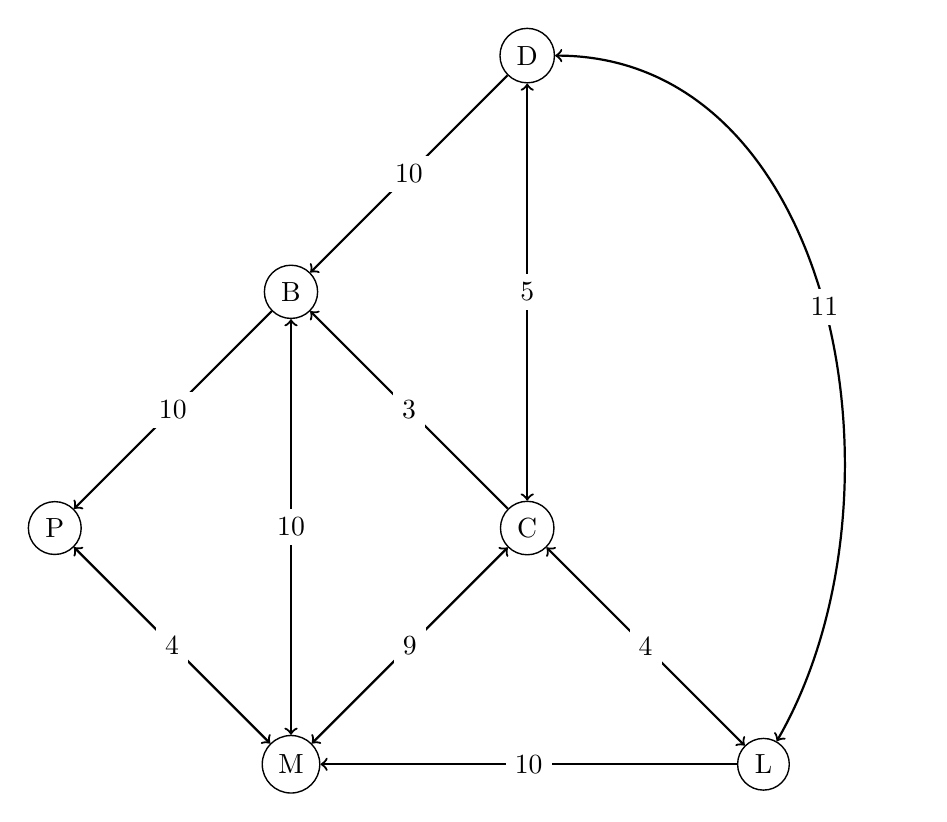
\begin{tikzpicture}
\GraphInit[vstyle=Normal] 
\SetGraphUnit{3}
\tikzset{VertexStyle/.append  style={fill}}
\Vertex{P}
\NOEA(P){B}  \SOEA(P){M} \NOEA(B){D}
\SOEA(B){C}  \SOEA(C){L}
\tikzset{EdgeStyle/.style={->}}
\Edge[label=$3$](C)(B)
\Edge[label=$10$](D)(B)
\Edge[label=$10$](L)(M)
\Edge[label=$10$](B)(P)
\tikzset{EdgeStyle/.style={<->}}
\Edge[label=$4$](P)(M)
\Edge[label=$9$](C)(M)
\Edge[label=$4$](C)(L)
\Edge[label=$5$](C)(D)
\Edge[label=$10$](B)(M)
\tikzset{EdgeStyle/.style={<->,relative=false,in=0,out=60}}
\Edge[label=$11$](L)(D)
\end{tikzpicture}
\begin{itemize}
	\item We always assume the weights of all edges are non-negative
	\item The \emph{weight} of a path is the sum of the weights of it's edges
	\item The \emph{shortest path-distance} from $u$ to $v$ is the minimum weight path from $u$ to $v$, denoted by $\delta(u, v)$
	\item Given a path $P$, a \emph{subpath} is any continuous segment of $P$.
	\item The triangle equality states that $\delta(x, z)$ must $\leq \delta(x, y) + \delta(y, z)$
	\item The \emph{shortest path problem} involves finding the shortest path from source vertex $s$ to \emph{all other vertices}.
\end{itemize}
\end{tcolorbox}
\vspace{1em}
\begin{algorithm}{Dijkstra's Algorithm}{Shortest Path Problem}{9}
	\item The algorithm computes an path-distance estimate to all vertices, denoted $d(v)$.
	\item A set $F$ of vertices is maintained which stores the shortest path-distances that have already been computed.
	\item Each iteration the algorithm picks the vertex not in $F$ with the smallest path-distance estimate $v$ and puts it in F - the intention is that this must now be the shortest path distance.
	\item Once $v$ is added to $F$, all estimates not in $F$ that are adjacent to $v$ are updated. This is called \emph{relaxation}.
	\item Let $G$ be the input graph and $s$ be the starting vertex.
		\begin{lstlisting}
set d(s) = 0 and d(v) = |$\infty$| where v is every other vertex, F = {s} and R = {every vertex that's not s}
	foreach v that has an edge outgoing from s, set d(v) to the weight of the edge between s and v
	while R contains a vertex with a distance < |$\infty$|
		select the vertex v in R with the lowest distance
		add v to F
		Relaxation: Update every vertex connected to a edge outgoing from v with new distance
		delete v from R
	endwhile
	\end{lstlisting}
	\item In order to construct the shortest path from $s$ to $u$, we find the edge ($a, u$) where $a$ is in F and is responsible for $u$ being put in F. We then do the same for $a$ until we end up at $s$.
	\item Dijkstra's runs in $O(e \log(v))$ time (where $v$ is the number of vertices and $e$ is the number of edges.) when using a heap data structure (see below)..
\end{algorithm}
\begin{tcolorbox}
	\section*{Priority Queue\hfill{LN9}}
	A priority queue data structure maintains a set $S$ of elements, where each $v$ in $S$ has a key - no two keys represent the same element but two elements may have the same key. The lower the value of the key, the higher the priority. The priority queue supports 3 operations - insert (add element), delete (remove element) and select (returns the element of the highest priority (ie. lowest key)).
	\section*{Heap\hfill{LN9}}
	Priority Queue data structures can be implemented using a heap, allowing for all operations to be completed in $O(\log n)$ time. A heap is a balanced binary (ie. 2 children nodes per parent) tree. Heaps are defined by the property that parents of any elements must have a key of equal or smaller value than their children. (ie. lowest keys at the top and largest at the bottom) This is called Heap order. We do insertion and deletion in a heap using HeapifyUp and HeapifyDown respectively.
\end{tcolorbox}
\begin{algorithm}{Heapify Up}{Heap Insertion}{9}
	\item Before running Heapify Up we insert the new entry into a leaf (ie. at the bottom of) of the existing tree.
	\item If the parent of the new entry has a key value lower than the new entry, do nothing
	\item If the parent has a higher key, swap the parent and the new entry. Then, run heapify up again on the entry and it's new parent.
	\item Since the height of the tree is $\log n$, the running time of the insert operation is $O(\log n)$.
\end{algorithm}
\begin{algorithm}{Heapify Down}{Heap Deletion}{9}
	\item Before running Heapify Down we insert the entry at the end of the tree into the ``hole'' left by the removed entry. If the key is too small for it's position just run Heapify Up. Otherwise, we need to run heapify Down.
	\item Intuitive. Check the new entry and it's two children and perform (or don't do anything) such that the entry out of the 3 with the smallest key is at ``top''.
	\item Need to descend at most $\log n$, so deletion is at most $O(\log n)$.
\end{algorithm}
\begin{tcolorbox}
\section*{Minimum Spanning Tree\hfill{LN10}}
Problem is intuitive: Given a weighted, undirected graph, find a tree that spans all vertices (ie. allows you to access all vertices) with the lowest possible total weight. A real life example would be if you were building a communications network between $n$ locations and you want to make sure they can all communicate to each other for the lowest cost of constructing the network.
\end{tcolorbox}
\begin{algorithm}{Prim}{Minimum Spanning Tree}{10}
	\item The assumption is made that no two edges have the same weight
	\item Start with a subset $V$ that only contains the starting vertex, $s$.
	\item Find an edge $e$ with the smallest weight such that one side of it is in $V$ and the other side is not.
	\item Add the vertex at the other end of the edge to $V$ and $e$ to $E$ ($E$ stores accepted edges)
	\item Running time is similar to Dijkstras, $e \log(v)$ ... why?
\end{algorithm}
\begin{algorithm}{Kruskal's}{Minimum Spanning Tree}{10}
	\item Start with just the vertices (and no edges) and add edges back one by one, in ascending order of weight. Skip edges that cause cycles.
	\item Running time is the same as Dijkstras and Prim, $e \log(v)$.
\end{algorithm}
\end{document}